% =============================================================================
%  PIDS - Proyecto 2: Sistema de detección de vehículos y conducción autónoma
%  Bloque 1: Recolección, anotación, análisis y depuración de datos
%
%  Compilar desde este directorio (guides/PIDS/semana-1):
%      pdflatex guide1.tex   (dos veces, para resolver las referencias)
% =============================================================================
\documentclass[12pt,a4paper]{article}

\usepackage[utf8]{inputenc}
\usepackage[a4paper, total={7in, 9.75in}, bottom=1in]{geometry}
\usepackage{amsmath}
\usepackage{graphicx}
\usepackage{caption}
\usepackage{subcaption}
\usepackage{framed}
\usepackage{hyperref}

% Rótulos en español (el documento lo está)
\renewcommand{\figurename}{Figura}
\renewcommand{\tablename}{Tabla}

\graphicspath{{./}{../}}

% ---------------- HEADER ----------------
\usepackage{fancyhdr}
\usepackage{graphicx}
\usepackage{xcolor}
\setlength{\headsep}{35pt}

\pagestyle{fancy}
\fancyhf{}

% Line
\renewcommand{\headrulewidth}{0.4pt}
\renewcommand{\headrule}{
\hbox to\headwidth{
  \color{gray}\leaders\hrule height \headrulewidth\hfill}
}

% Center (left header)
\fancyhead[L]{
    \begin{minipage}{10cm}
        \scriptsize \textbf{Proyectos en Ingeniería de Datos y Sistemas (PIDS)}\\
        \scriptsize Proyecto 2: Sistema de detección de vehículos y conducción autónoma
    \end{minipage}
}

% Right: group/university + logo aligned horizontally
\fancyhead[R]{
    \begin{minipage}{5.2cm}
        \scriptsize \textbf{Universidad Politécnica de Madrid}\\
        \scriptsize Grupo de Tratamiento de Imágenes
    \end{minipage}
    \raisebox{-0.3\height}{
        
\includegraphics[height=0.8cm]{header/logo_upm.pdf}
    }
}


\begin{document}

% =============================================================================
%  Título
% =============================================================================
\begin{center}
    \vspace*{.15cm}
    {\Huge \bfseries Bloque 1: Recolección, anotación, análisis y depuración de datos} \\[0.5cm]
\end{center}


% =============================================================================
\section{Introducción}
% =============================================================================

A lo largo de este proyecto desarrollaremos una red neuronal para la detección de objetos en imágenes, más concretamente, de \underline{\textbf{RoboMasters}} adversarios (figura~\ref{fig: RoboMaster}). En este primer bloque construiremos el conjunto de datos con el que aprenderá la red, siguiendo cuatro pasos:

\begin{itemize}
    \item \underline{\textbf{Recolección:}} los datos son el alimento de las redes neuronales, y su calidad determina en gran medida la capacidad de la red para generalizar.
    \item \underline{\textbf{Anotación:}} etiquetar los datos para que la red pueda aprender de ellos. Una anotación incorrecta o inconsistente lleva directamente a un modelo defectuoso.
    \item \underline{\textbf{Análisis exploratorio y aumento de datos:}} entender qué contienen realmente nuestros datos, detectar sesgos o ampliar la cantidad de datos con transformaciones que simulen situaciones no capturadas.
    \item \underline{\textbf{Depuración:}} eliminar los datos incorrectos o irrelevantes que perjudicarían al entrenamiento.
\end{itemize}


% =============================================================================
\section{Recolección de datos}
% =============================================================================

Como el objetivo final es detectar RoboMasters adversarios desde el propio robot, los datos deberemos capturarlos también desde el mismo. El primer paso es conectarnos al RoboMaster desde un dispositivo móvil (Android o iOS):

\begin{enumerate}
    \item Descargue la aplicación ``\textit{RoboMaster}'', disponible en la \href{https://apps.apple.com/us/app/robomaster/id1449678340}{\underline{App Store}} (iOS) o en este \href{https://upm365-my.sharepoint.com/:u:/g/personal/d_fcoiras_upm_es/EdBzFP_mAq5OhpeC3TUAZJQBiR4BNGKcqP7WRSZRQq55SQ?e=0goYev}{\underline{enlace}} (Android).
    \item Encienda el robot y asegúrese de que la pestaña deslizante de su cabeza apunta al símbolo de un dispositivo móvil (figura~\ref{fig: Wi-Fi module}).
    \item Conéctese a la Wi-Fi que emite el RoboMaster. Su nombre y contraseña están impresos en la parte superior de la cabeza del robot (figura~\ref{fig: Wi-Fi module}).
    \item Con la Wi-Fi conectada, ya puede abrir la aplicación y controlar el robot.
\end{enumerate}

\begin{framed}
    \centering
    \textbf{IMPORTANTE}: la aplicación preguntará si queremos actualizar el firmware. Dadle a \underline{\textbf{NO}}.
\end{framed}

\begin{figure}[t]
\centering
    \begin{subfigure}{0.5\textwidth}
        \centering
        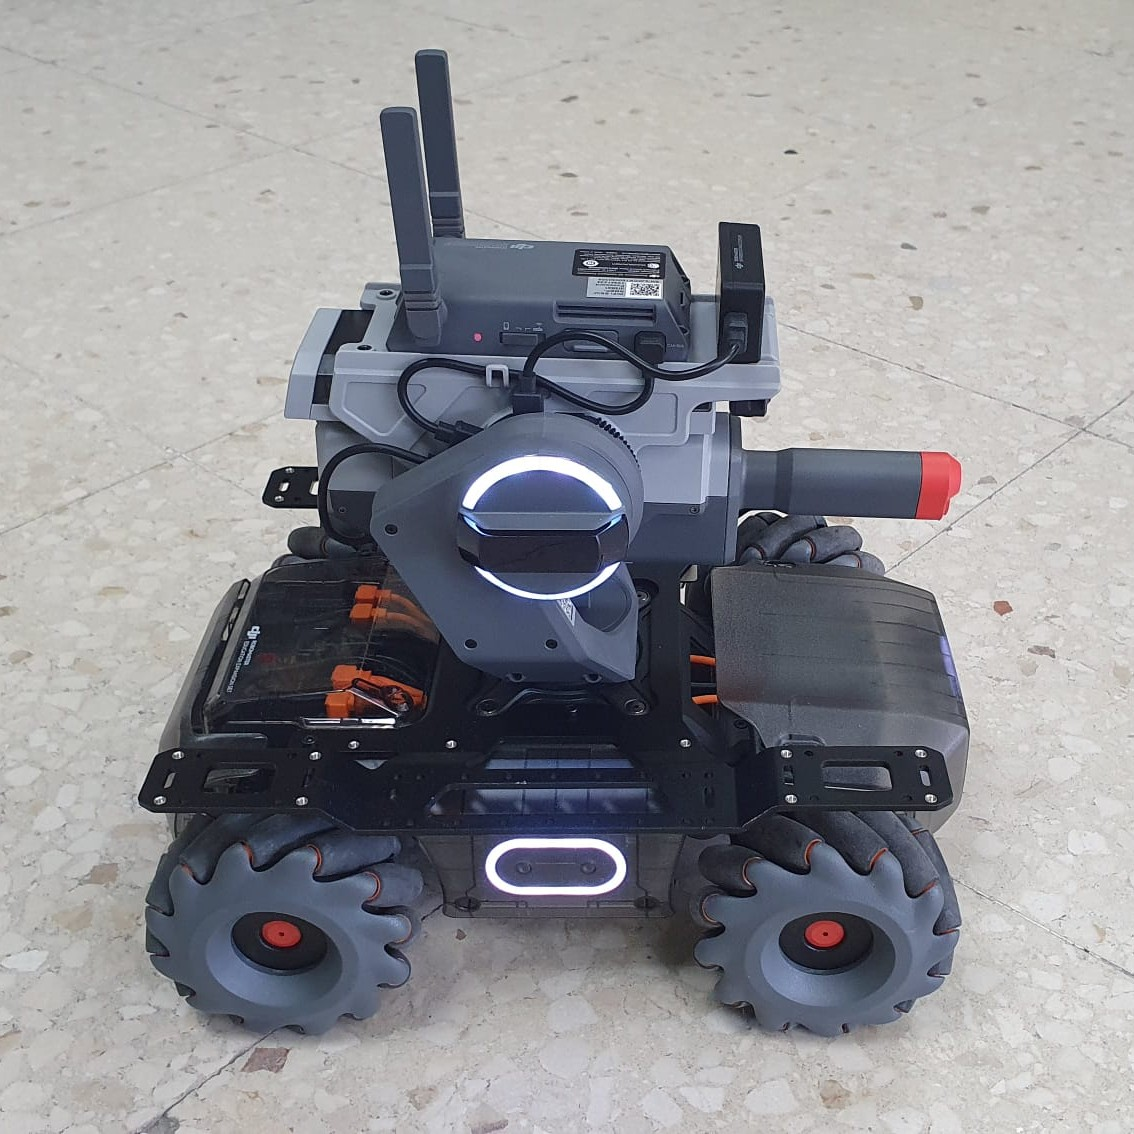
\includegraphics[width=\textwidth]{images1/robot.jpg}
        \caption{RoboMaster}
        \label{fig: RoboMaster}
    \end{subfigure}\hfill
    \begin{subfigure}{0.5\textwidth}
        \centering
        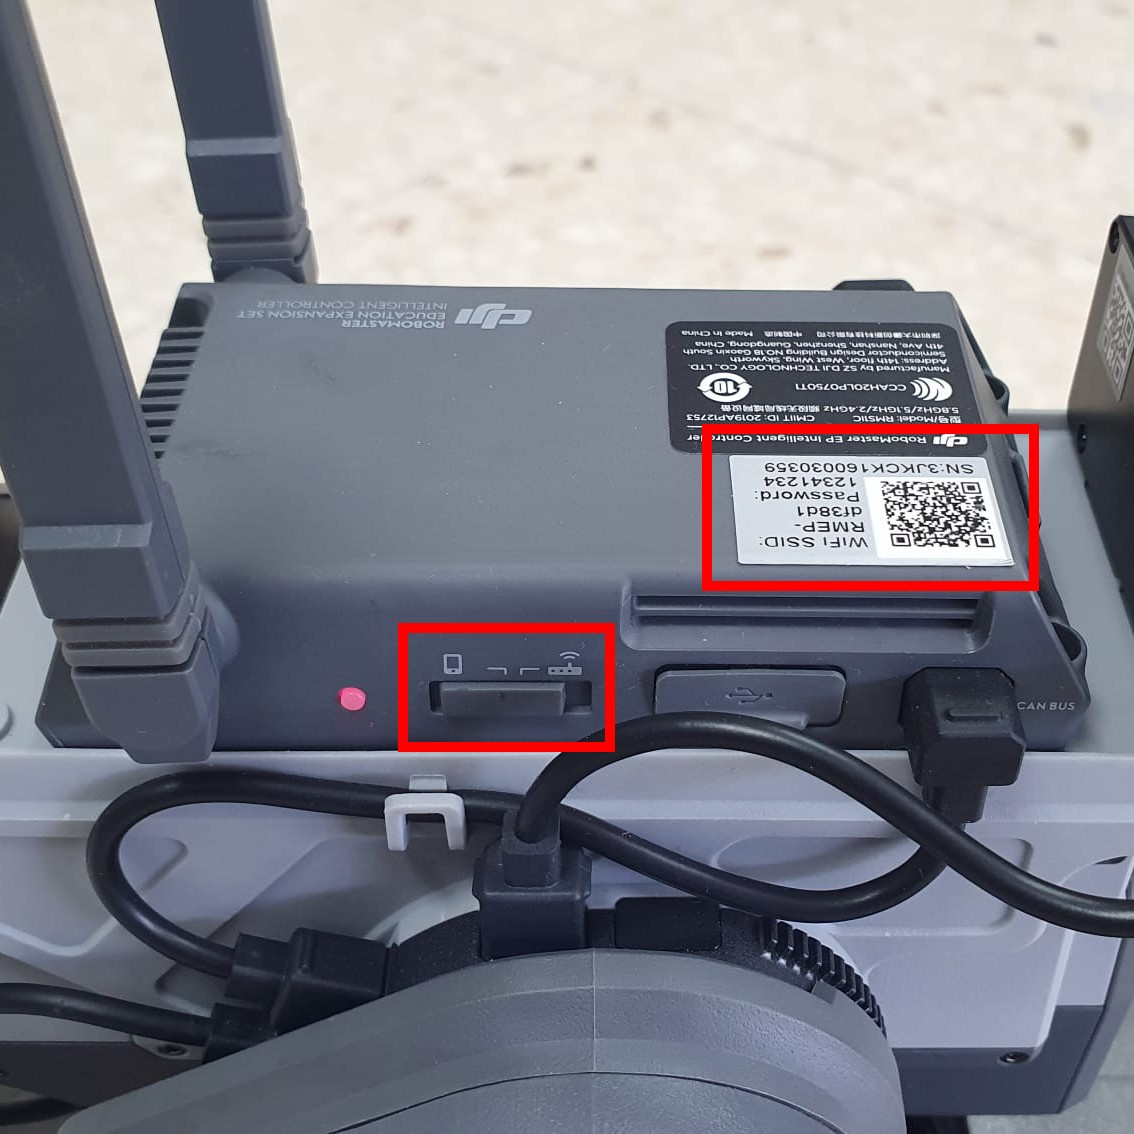
\includegraphics[width=\textwidth]{images1/robot-wifi.jpg}
        \caption{Módulo Wi-Fi}
        \label{fig: Wi-Fi module}
    \end{subfigure}
    \caption{RoboMaster y su módulo Wi-Fi.}
    \label{fig: RoboMaster y su módulo Wi-Fi}
\end{figure}

\begin{figure}[t]
\centering
    \begin{subfigure}{0.7\textwidth}
        \centering
        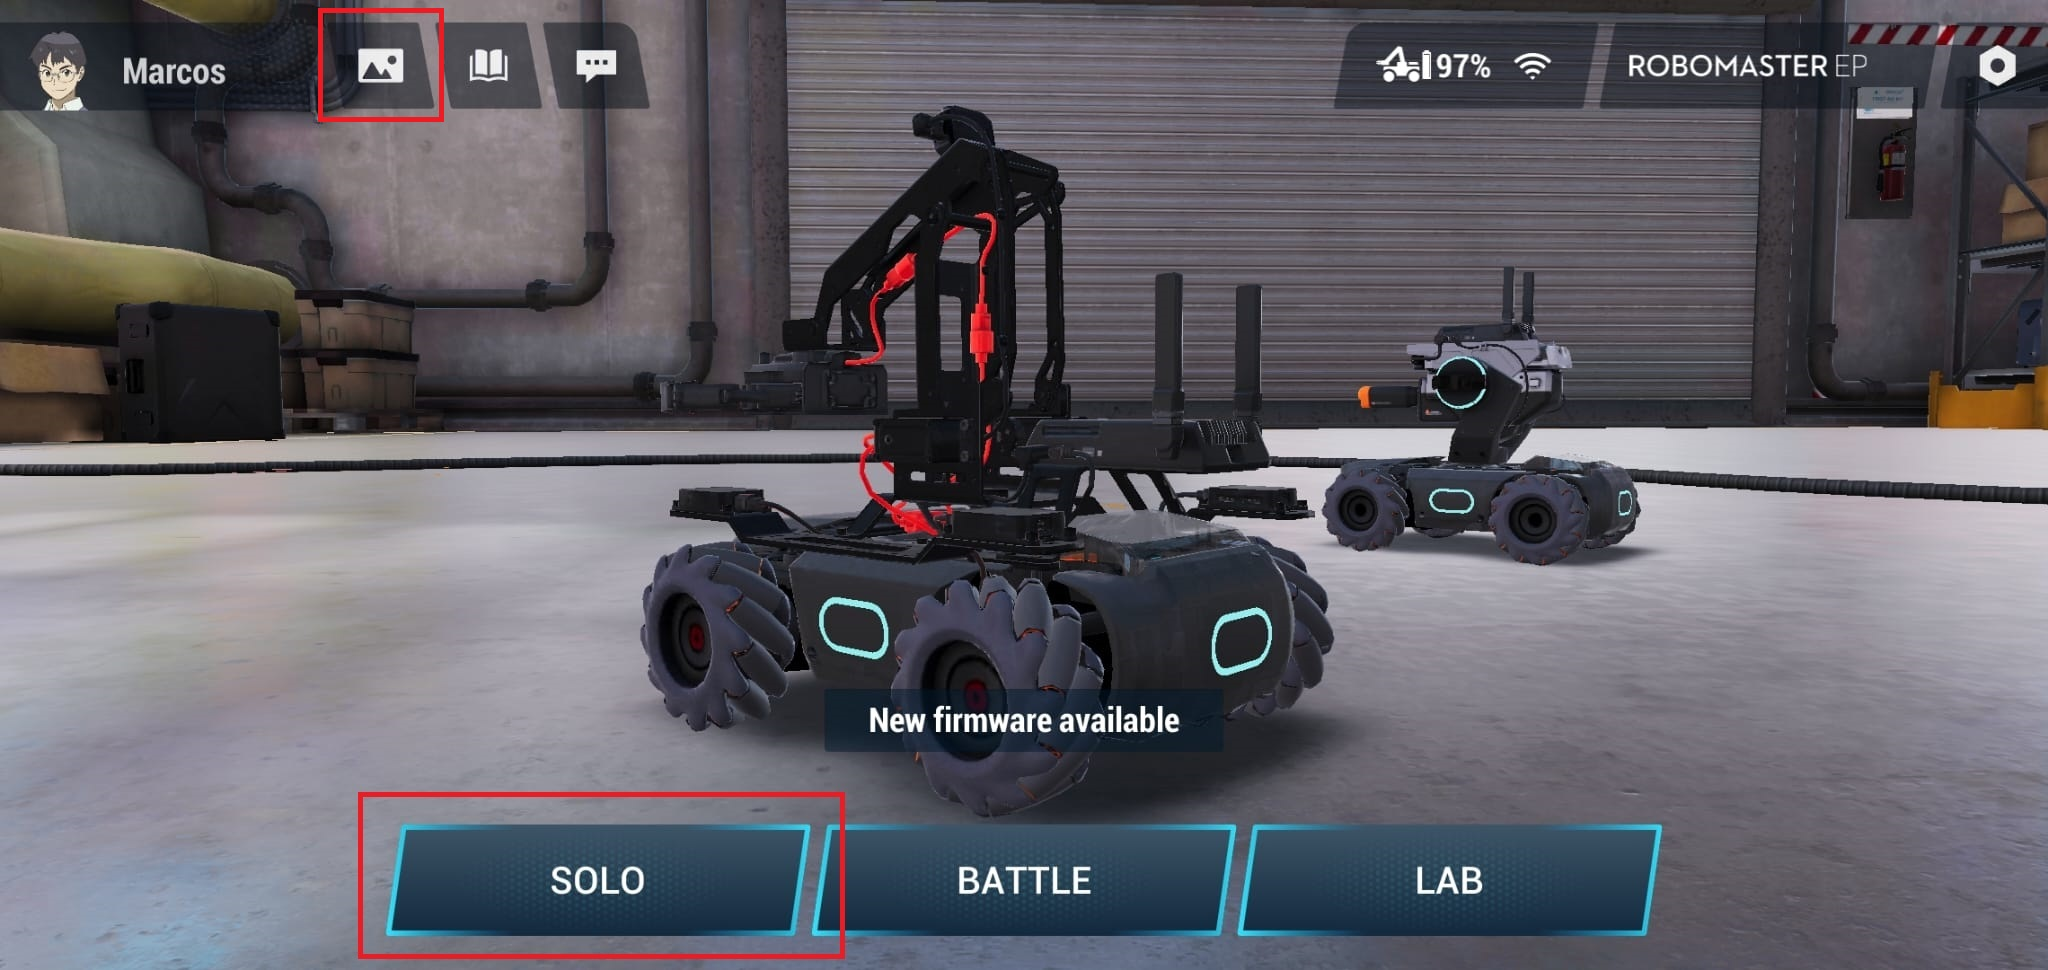
\includegraphics[width=\textwidth]{images1/robot-menu.jpeg}
        \caption{Menú de inicio}
        \label{fig: Menú de inicio}
    \end{subfigure}\hfill
    \begin{subfigure}{0.7\textwidth}
        \centering
        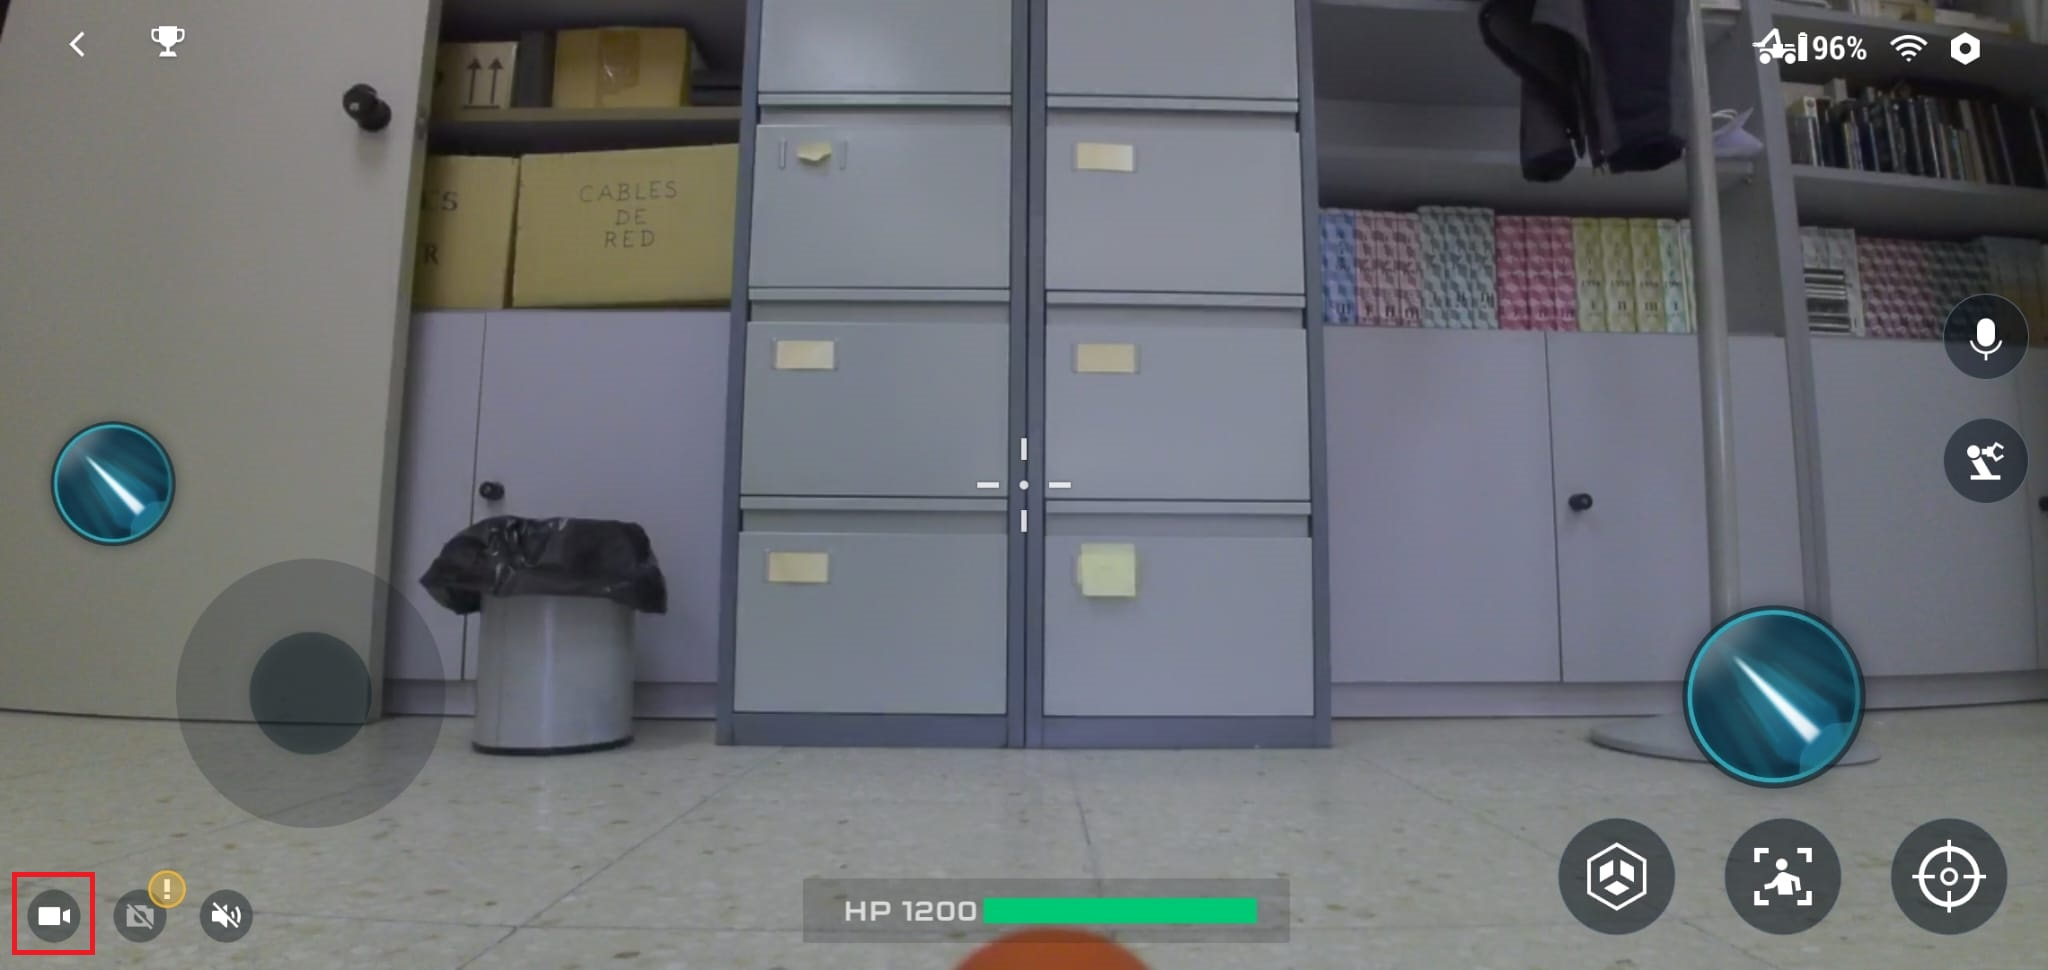
\includegraphics[width=\textwidth]{images1/robot-solo.jpeg}
        \caption{Interfaz gráfica de un solo jugador}
        \label{fig: Interfaz de un solo jugador}
    \end{subfigure}
    \caption{Menú de inicio e interfaz de un solo jugador del RoboMaster.}
    \label{fig: Menú de inicio e interfaz de un solo jugador del RoboMaster}
\end{figure}

Cada grupo se conectará a un RoboMaster y grabará vídeo desde él mientras los robots se desplazan por el entorno, procurando que al menos un RoboMaster adversario aparezca siempre en la escena. De esos vídeos extraeremos después las imágenes que anotaremos.

Para grabar (figura~\ref{fig: Menú de inicio e interfaz de un solo jugador del RoboMaster}), pulse el botón ``Solo'' para tomar el control del robot (figura~\ref{fig: Menú de inicio}) y, ya en la interfaz de conducción, el botón de captura de vídeo de la esquina inferior izquierda (figura~\ref{fig: Interfaz de un solo jugador}). Durante la captura, trate de variar:

\begin{itemize}
    \item la iluminación de la escena;
    \item la oclusión de los RoboMasters;
    \item el contexto y el fondo del escenario;
    \item la posición y orientación de los RoboMasters;
    \item la distancia a la que aparecen y el movimiento de la cámara.
\end{itemize}

Recuerde que recolectar datos no consiste solo en obtener muchos, sino en que sean \textbf{representativos} del problema. Si solo grabamos en interiores, la red fallará en exteriores; si nunca hay oclusiones, será incapaz de detectar robots parcialmente ocultos.

Anote también la duración, la resolución y la tasa de imágenes por segundo de cada vídeo: los necesitará para el informe.

Para descargar los vídeos, entre en la galería desde el menú de inicio (figura~\ref{fig: Menú de inicio}) pulsando el icono de la esquina superior izquierda; al seleccionar un vídeo aparecerá un botón de descarga en la esquina superior derecha. No olvide poner un nombre adecuado a cada vídeo (``video1.mp4, video2.mp4, ...'' o ``lab.mp4, pasillo.mp4, ...'').

% -----------------------------------------------------------------------------
\subsection{JupyterHub}
% -----------------------------------------------------------------------------

Gran parte del proyecto se realizará sobre una plataforma JupyterHub, con la excepción de la herramienta de anotación y del control por código del RoboMaster. Acceda a \url{https://k8ssr.labdoc.ssr.upm.es:30000} (figura~\ref{fig: Ventana de login}) con:

\begin{itemize}
    \item \textbf{Username}: pidsX (donde X es el número de grupo).
    \item \textbf{Password}: pids2026
\end{itemize}

Tras autenticarse, seleccione el perfil \underline{PIDS} (figura~\ref{fig: Selección de perfil}) y accederá a la interfaz de JupyterHub (figura~\ref{fig: Interfaz de JupyterHub}).

\begin{figure}[t]
\centering
    \begin{subfigure}{0.5\textwidth}
        \centering
        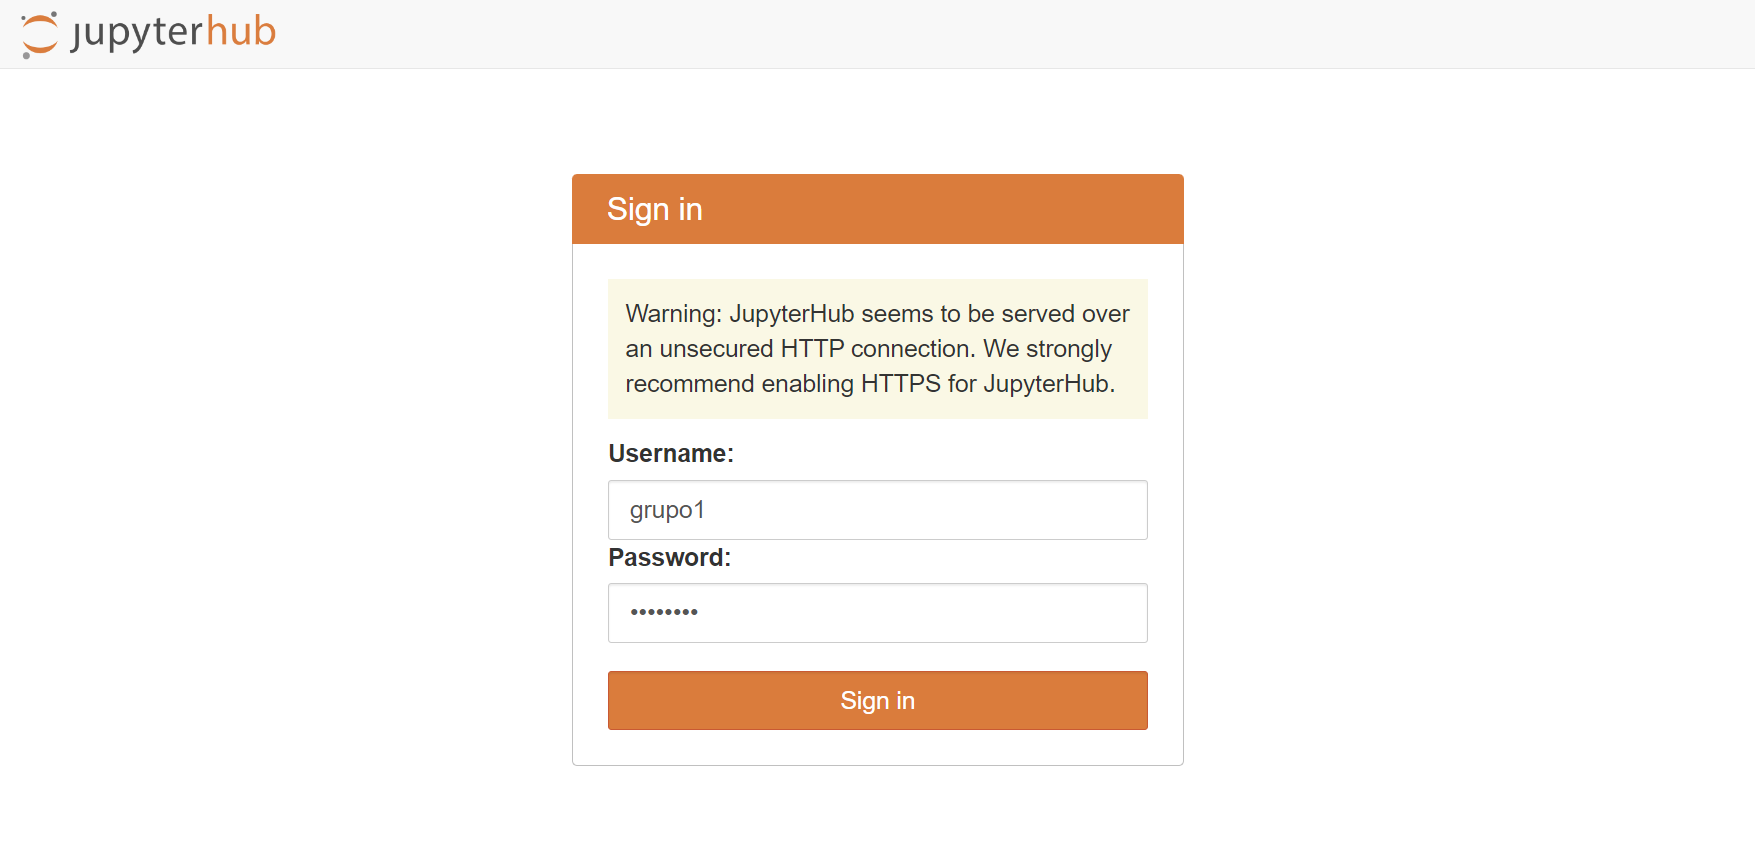
\includegraphics[width=\textwidth]{images1/jupyterhub-login.png}
        \caption{Ventana de login}
        \label{fig: Ventana de login}
    \end{subfigure}\hfill
    \begin{subfigure}{0.5\textwidth}
        \centering
        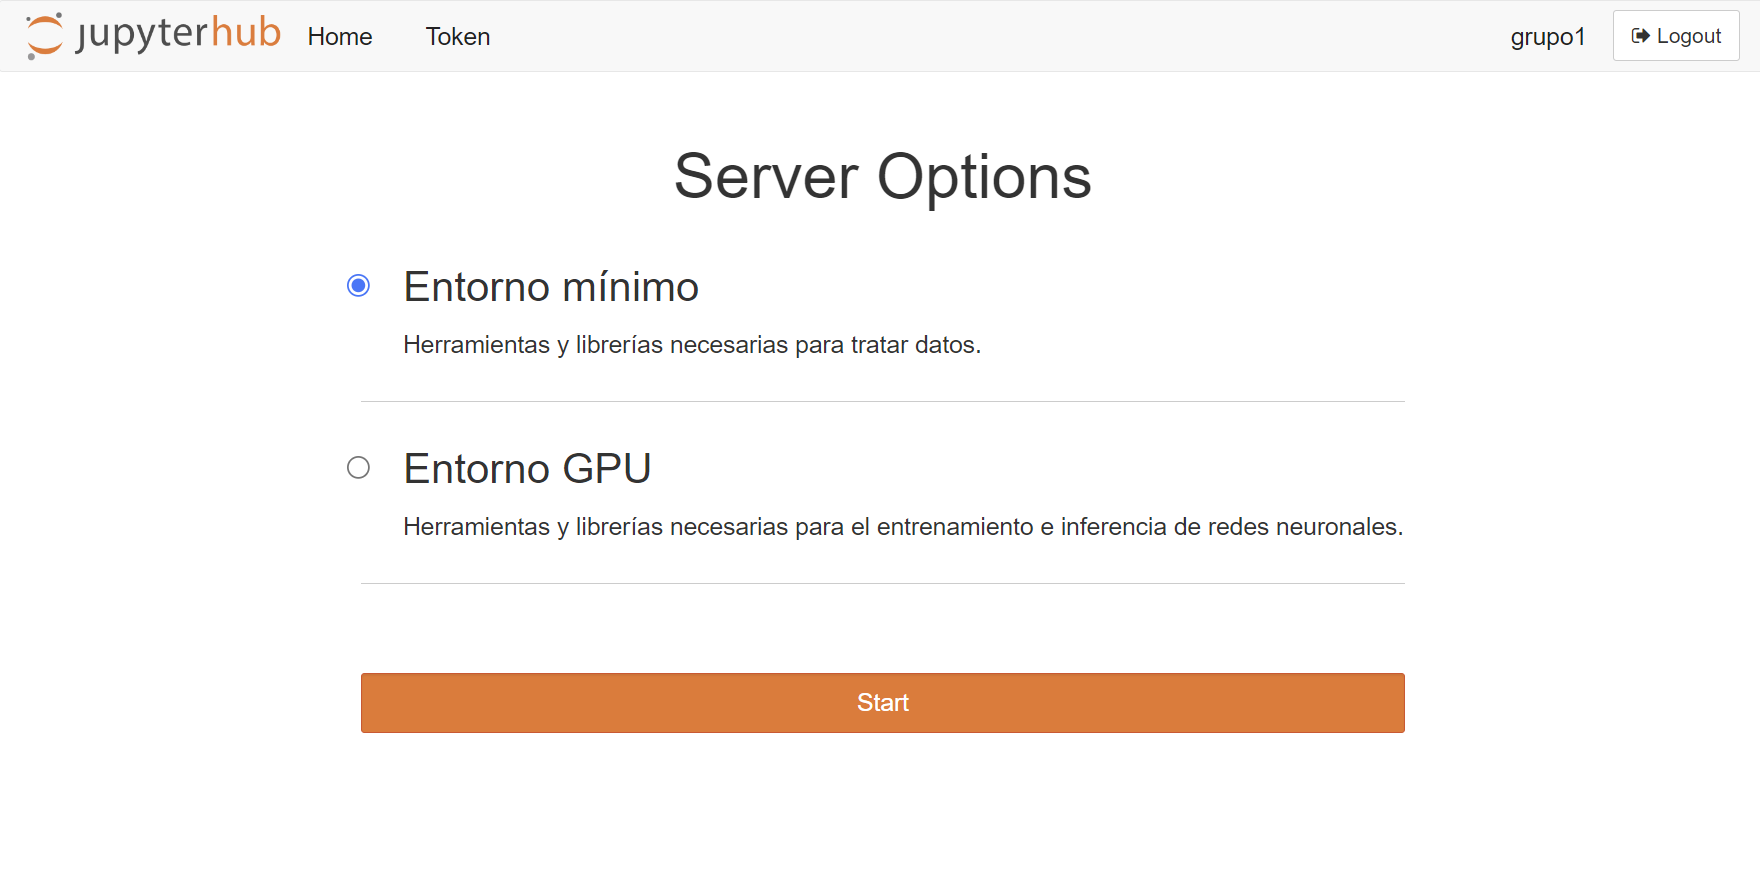
\includegraphics[width=\textwidth]{images1/jupyterhub-profiles.png}
        \caption{Selección de perfil}
        \label{fig: Selección de perfil}
    \end{subfigure}
    \begin{subfigure}{0.5\textwidth}
        \centering
        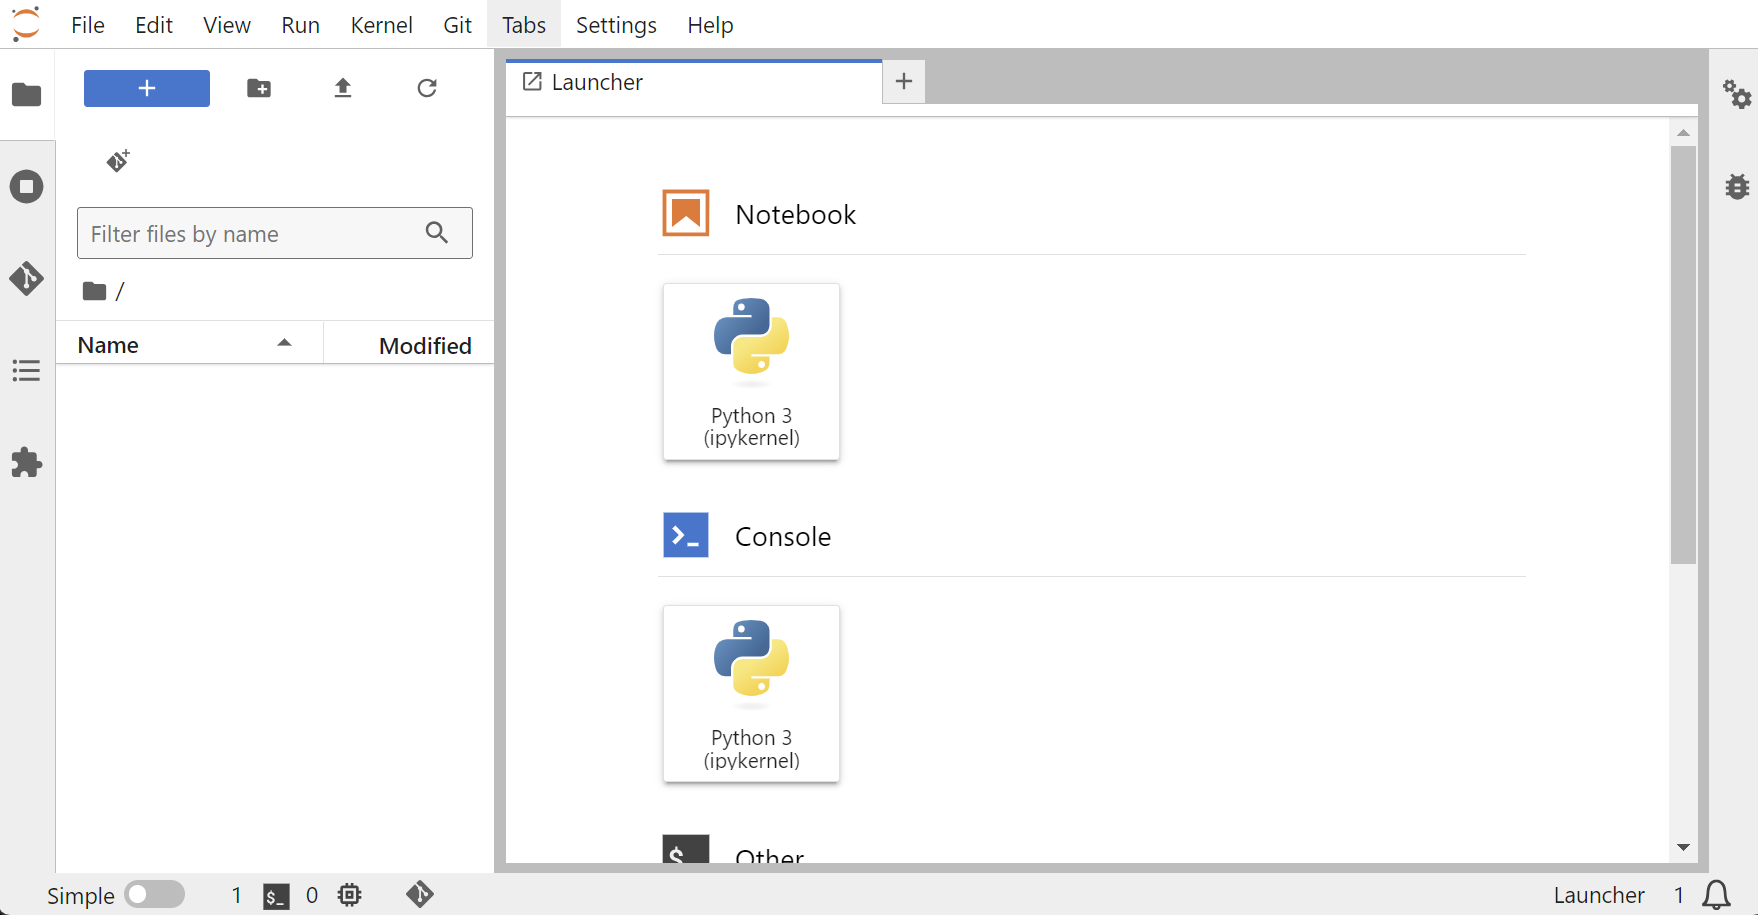
\includegraphics[width=\textwidth]{images1/jupyterhub-ui.png}
        \caption{Interfaz de JupyterHub}
        \label{fig: Interfaz de JupyterHub}
    \end{subfigure}
    \caption{Pantallas de acceso a la interfaz de JupyterHub.}
    \label{fig: Pantallas de acceso a la interfaz de JupyterHub}
\end{figure}

Los perfiles ya vienen poblados con la estructura del proyecto: los guiones de prácticas (\textit{guides}), los notebooks (\textit{week1}, \textit{week2}) y los datos de validación y test (\textit{data\_val}, \textit{data\_test}).

Esta semana trabajaremos con los notebooks de \textit{week1}, empezando por \underline{video2frames.ipynb}. Antes de ejecutarlo, suba los vídeos grabados a una nueva carpeta \textit{data\_train}. Preste especial atención a la variable \textit{INTERVAL}, que fija cada cuántos fotogramas se extrae una imagen y, por tanto, cuántas imágenes obtendrá:

\begin{equation*}
    \text{n\'umero de im\'agenes} \approx
    \frac{\text{fps} \times \text{duraci\'on total (s)}}{\mathit{INTERVAL}}
\end{equation*}

Elija su valor a partir de los fps de sus vídeos y del número de imágenes deseado (en torno a 800). Al ejecutar el notebook obtendrá una carpeta por vídeo, cada una con los subdirectorios ``images'' y ``labels'': las imágenes extraídas y, tras la sección~\ref{sec: Anotación de datos}, sus anotaciones.


% =============================================================================
\section{Anotación de datos}
\label{sec: Anotación de datos}
% =============================================================================

\begin{figure}[t]
    \centering
    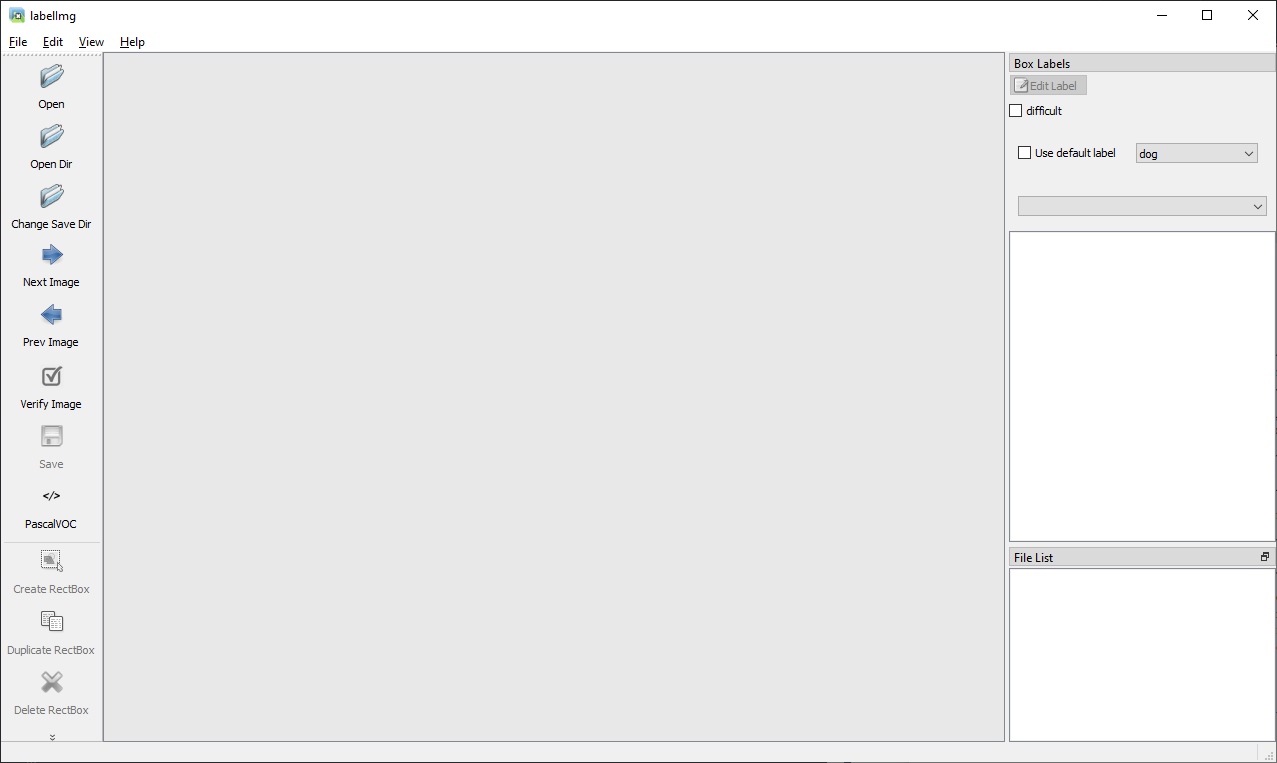
\includegraphics[width=0.85\textwidth]{images1/labelimg.png}
    \caption{Interfaz gráfica de la herramienta de anotación \textit{labelImg}.}
    \label{fig: labelImg}
\end{figure}

Anotar consiste en marcar, en cada imagen, los ``bounding boxes'' de los objetos que queremos detectar. La red aprenderá de esas imágenes y de sus anotaciones, así que estas deben ser no solo precisas, sino también \textbf{consistentes} entre todos los miembros del grupo.

Usaremos \textit{labelImg}, que ofrece una interfaz gráfica para dibujar las cajas. Como esa interfaz no puede abrirse en JupyterHub, tendremos que descargar el conjunto de datos, anotarlo en local y volver a subirlo.

% -----------------------------------------------------------------------------
\subsection{Carga y descarga de datos en JupyterHub}
% -----------------------------------------------------------------------------

En JupyterHub se pueden subir archivos arrastrándolos desde el explorador local, y descargarlos con click derecho $\rightarrow$ ``Descargar''. Sin embargo, \textbf{no admite carpetas}, solo archivos sueltos. Para descargar una carpeta hay que comprimirla antes desde un terminal (Ctrl+Shift+L $\rightarrow$ Terminal):

\begin{verbatim}
    zip -r <nombre-archivo>.zip /path/a/mis/datos
\end{verbatim}

Ya comprimida, puede descargarla como cualquier otro archivo y descomprimirla con cualquier herramienta (Winrar, 7zip, etc.) o, en Linux, con:

\begin{verbatim}
    unzip <nombre-archivo>.zip
\end{verbatim}

Para subir una carpeta, haga el camino inverso: suba el .zip y descomprímalo en el terminal de JupyterHub.

\begin{framed}
    \centering
    \textbf{Nota:} tampoco se pueden eliminar carpetas desde el panel izquierdo; hay que usar ``rm -r /path/a/la/carpeta''. MUCHO CUIDADO con lo que se borra: mantenga siempre una copia del conjunto de datos y del código.
\end{framed}

% -----------------------------------------------------------------------------
\subsection{(Opcional) Instalación de labelImg}
% -----------------------------------------------------------------------------

Solo si desea anotar desde casa. \underline{En los ordenadores del laboratorio ya está instalada}.

\begin{itemize}
    \item \textbf{Windows:} instale \href{https://www.anaconda.com/download/success}{Anaconda} y ejecute en su terminal:
        \begin{verbatim}
            conda create -n venv python=3.7
            conda activate venv
            git clone https://github.com/HumanSignal/labelImg.git
            conda install pyqt=5
            conda install -c anaconda lxml
            pip install pyqt5-tools opencv-python
            cd labelImg
            pyrcc5 -o libs/resources.py resources.qrc
            python labelImg.py
        \end{verbatim}

    \item \textbf{Linux:} instale Python 3.8 si no lo tiene (tres primeros comandos), cree un entorno virtual e instale labelImg (cuatro últimos):
        \begin{verbatim}
            sudo add-apt-repository ppa:deadsnakes/ppa
            sudo apt update
            sudo apt install -y python3.8 python3.8-venv

            python3.8 -m venv venv
            source venv/bin/activate
            pip install labelImg==1.8.6
            labelImg
        \end{verbatim}
\end{itemize}
\vspace{-1cm}

% -----------------------------------------------------------------------------
\subsection{Uso de labelImg}
% -----------------------------------------------------------------------------

En el laboratorio, abra un terminal y ejecute:

\begin{verbatim}
    cd /home/PIDS/robomaster
    ./labelimg/labelimg.sh
\end{verbatim}

La interfaz es bastante intuitiva (figura~\ref{fig: labelImg}). Antes de empezar, configúrela así:

\begin{enumerate}
    \item ``Open Dir'': seleccione la carpeta con las imágenes a etiquetar (\textit{/path/al/dataset/videoX/images}).
    \item ``Change Save Dir'': seleccione la carpeta \textit{labels} asociada, donde se guardarán las anotaciones (\textit{/path/al/dataset/videoX/labels}).
    \item Menú ``View'' $\rightarrow$ ``Single Class Mode'', ya que solo tenemos una clase.
\end{enumerate}

Para anotar, pulse ``Create RectBox'' (atajo \textit{w}) y dibuje la caja; la primera vez se le pedirá un nombre de clase, escriba ``robot''. Cuando haya marcado todos los robots de la imagen, guarde (\textit{CTRL+s}) y pase a la siguiente (\textit{d}). El resultado debe parecerse al de la figura~\ref{fig: annotation example}.

\begin{figure}[t]
    \centering
    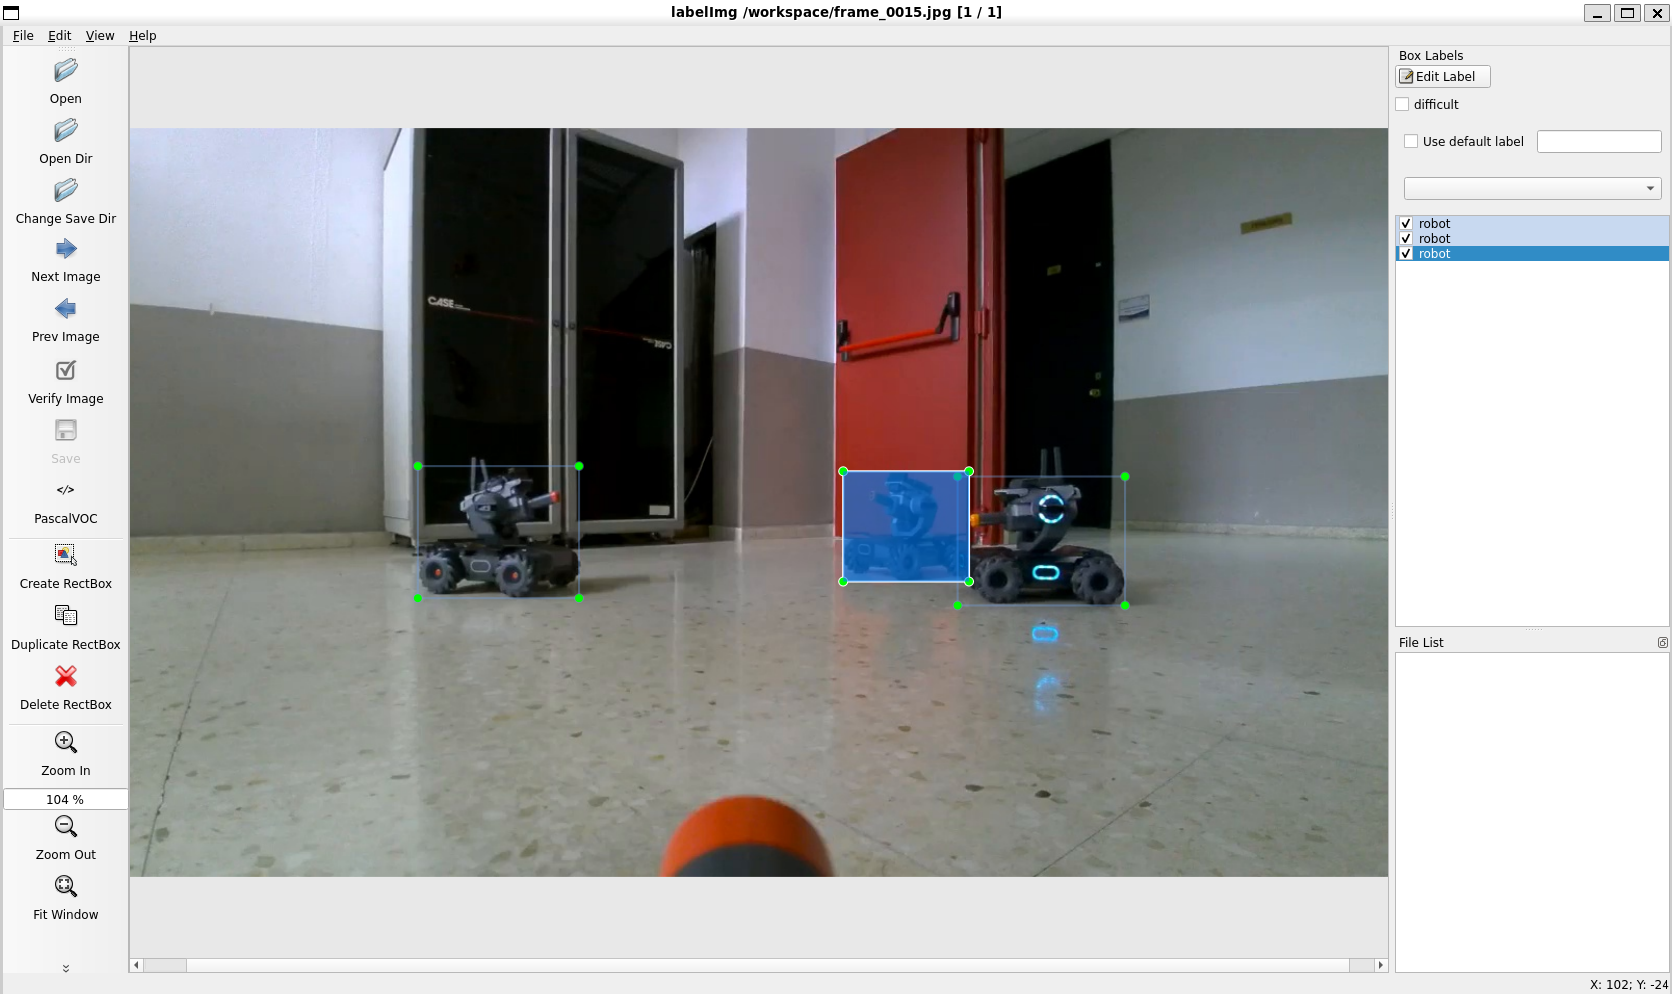
\includegraphics[width=\textwidth]{images1/labelimg-example.png}
    \caption{Ejemplo de anotación con la herramienta \textit{labelImg}.}
    \label{fig: annotation example}
\end{figure}

La red aprenderá a dibujar las cajas \textbf{exactamente como usted las dibuje}: si las ajusta muy ceñidas al robot, sus predicciones también lo estarán. Antes de empezar, acuerde con su grupo unos criterios comunes y anótelos, porque tendrá que justificarlos en el informe: ¿se anotan los robots parcialmente ocluidos, y a partir de qué porcentaje visible? ¿Y los que aparecen muy lejanos, desenfocados o cortados por el borde de la imagen?


% =============================================================================
\section{Análisis exploratorio de los datos (EDA)}
% =============================================================================

El análisis exploratorio (EDA) sirve para comprobar que el conjunto de datos está listo para entrenar, para detectar problemas y para tomar decisiones informadas. Entre las técnicas más habituales están:

\begin{itemize}
    \item \textbf{Visualización de imágenes}, para examinar su calidad, su variabilidad y posibles defectos como el desenfoque o las distorsiones.
    \item \textbf{Visualización de las anotaciones} superpuestas a las imágenes, para comprobar que las cajas están bien alineadas con los robots.
    \item \textbf{Estadísticas básicas}: número de imágenes, tamaño medio de las imágenes, distribución del tamaño de los bounding boxes, etc.
    \item \textbf{Distribución por clases o escenarios}: ¿hay un equilibrio razonable entre imágenes con y sin robots, y entre los distintos escenarios? Un desequilibrio introduce sesgos en el detector.
\end{itemize}

La figura~\ref{fig: Ejemplos de los análisis exploratorios} muestra algunos ejemplos. El notebook \textit{eda.ipynb} es solo un punto de partida: se espera que amplíe el análisis por su cuenta de cara al entregable (sección~\ref{sec:objetivos}).

\begin{figure}[t]
\centering
    \begin{subfigure}{0.5\textwidth}
        \centering
        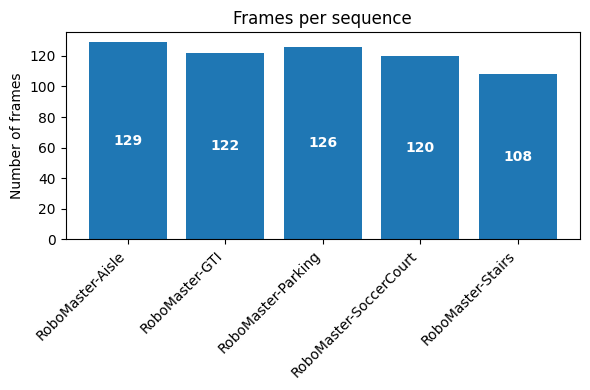
\includegraphics[width=\textwidth]{images1/eda-frames.png}
    \caption{Distribución de imágenes por secuencia}
    \label{fig: Distribución de imágenes por secuencia}
    \end{subfigure}\hfill
    \begin{subfigure}{0.5\textwidth}
        \centering
        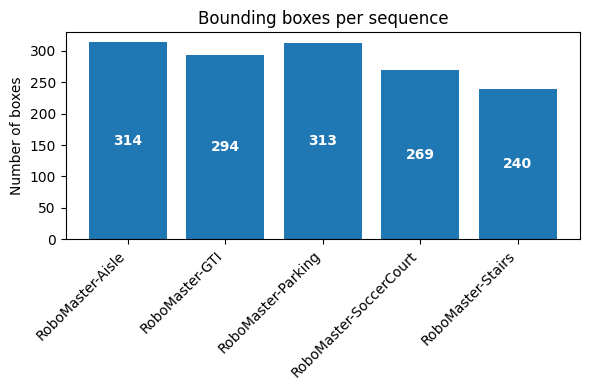
\includegraphics[width=\textwidth]{images1/eda-bboxes.png}
    \caption{Distribución de bounding boxes por secuencia}
    \label{fig: Distribución de bounding boxes por secuencia}
    \end{subfigure}\hfill
    \begin{subfigure}{1.0\textwidth}
        \centering
        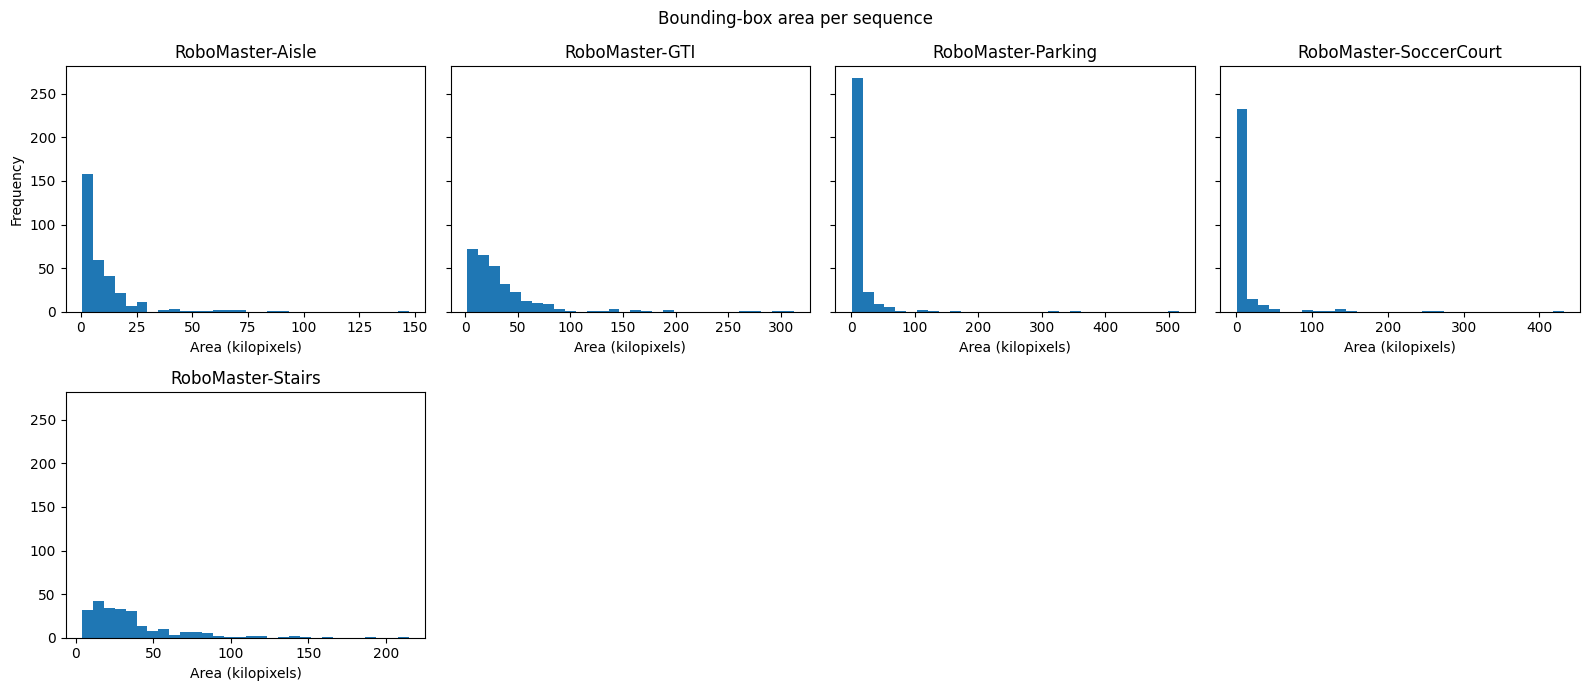
\includegraphics[width=\textwidth]{images1/eda-bboxes-area.png}
    \caption{Distribución del área de los bounding boxes por secuencia}
    \label{fig: Distribución del area de los bounding boxes por secuencia}
    \end{subfigure}\hfill
    \begin{subfigure}{1.0\textwidth}
        \centering
        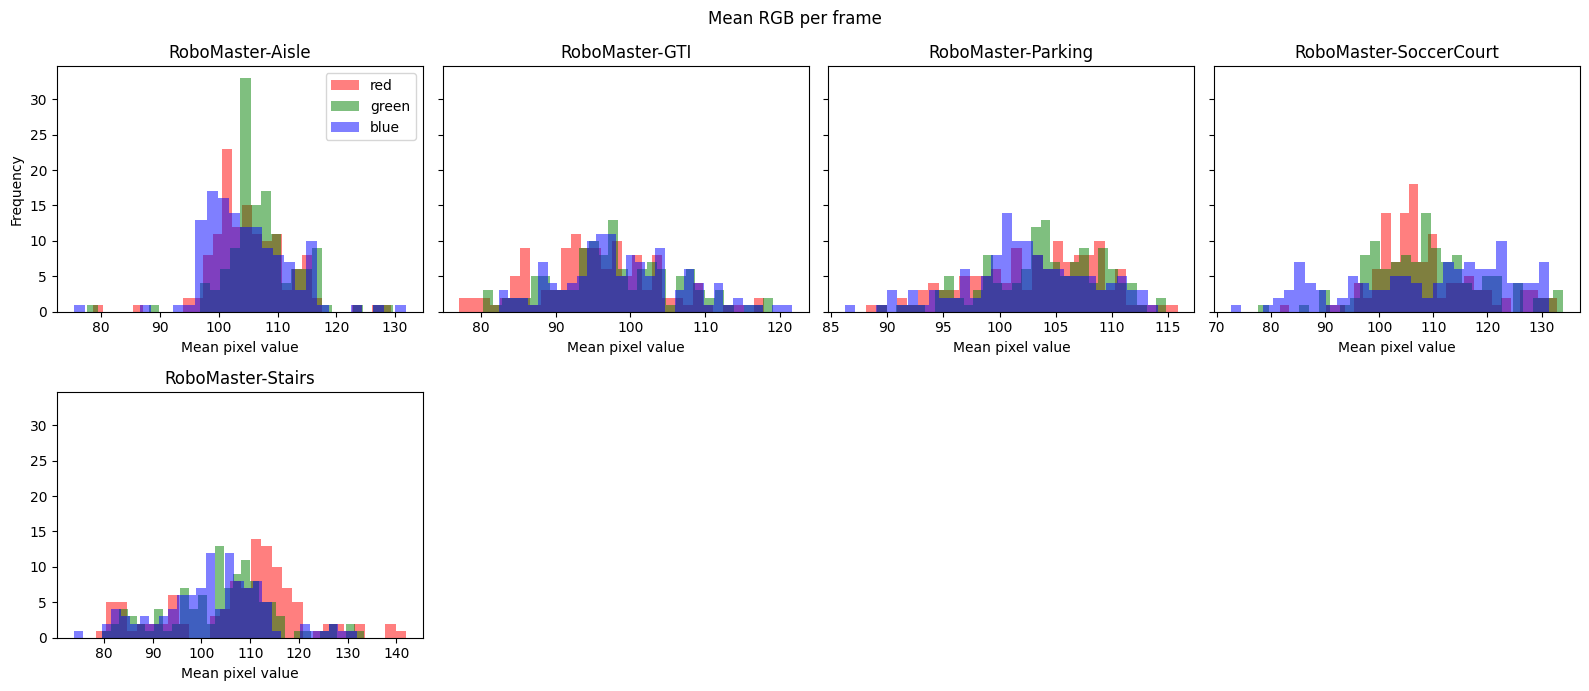
\includegraphics[width=\textwidth]{images1/eda-rgb.png}
    \caption{Distribución de canales RGB por secuencia}
    \label{fig: Distribución de canales RGB por secuencia}
    \end{subfigure}
    \caption{Ejemplos de análisis exploratorios de datos.}
    \label{fig: Ejemplos de los análisis exploratorios}
\end{figure}


% =============================================================================
\section{Aumento de datos (\textit{data augmentation})}
% =============================================================================

Grabar y anotar imágenes es lento, pero podemos multiplicar las que ya tenemos generando copias modificadas: volteos, recortes, desenfoques, cambios de brillo o de color... Cada copia le parece distinta al modelo y, sin embargo, muestra la misma escena, de modo que la red aprende a ser \textbf{robusta} frente a esos cambios en lugar de memorizar las imágenes de entrenamiento.

El notebook \textit{data\_aug.ipynb} implementa este proceso con la librería \textit{albumentations}. Dos ideas a tener en cuenta:

\begin{itemize}
    \item \textbf{Las anotaciones acompañan a la imagen}: al voltear o recortar una imagen hay que transformar también sus bounding boxes. La librería se encarga de ello.
    \item \textbf{Solo se aumentan los datos originales}, nunca los ya aumentados: acumular distorsión sobre distorsión no añade información.
\end{itemize}

Elegir las transformaciones no es automático: cada una debe simular una variabilidad que el robot vaya a encontrarse de verdad. Un volteo horizontal es razonable, pero uno vertical implicaría ver un robot terrestre boca abajo. Consulte el catálogo completo en \url{https://albumentations.ai/explore/} y \url{https://albumentations.ai/docs/api-reference/}.


% =============================================================================
\section{Depuración de datos}
% =============================================================================

Depurar consiste en revisar los datos capturados y anotados para identificar y corregir problemas: imágenes defectuosas, mal etiquetadas o que no aportan valor. Entrenar con datos erróneos o ruidosos degrada de forma notable el rendimiento del modelo final.

Busque, por ejemplo, imágenes con etiquetas incorrectas, imágenes en las que el robot está anotado pero no es realmente visible, imágenes casi idénticas entre sí, o situaciones poco representativas que puedan sesgar el aprendizaje. Tenga en cuenta el riesgo contrario: si elimina todos los casos difíciles, obtendrá un conjunto fácil y un modelo que falla en la realidad.


% =============================================================================
\section{Objetivos}
\label{sec:objetivos}
% =============================================================================

Al terminar este bloque, cada grupo deberá haber conseguido lo siguiente:

\begin{itemize}
    \item \textbf{Datos:} capturar y anotar al menos 800 imágenes. Evite un número mucho mayor: alargará innecesariamente la anotación y el entrenamiento del Bloque 2.
    \item \textbf{Análisis exploratorio:} aplicar el análisis de \textit{eda.ipynb} a sus datos e \underline{incluir algún análisis adicional}, justificando qué pregunta responde y qué ha revelado.
    \item \textbf{Aumento de datos:} entender qué transformaciones aplica \textit{data\_aug.ipynb} y por qué unas sí y otras no. Ajustar la lista de transformaciones a conveniencia, \underline{añadiendo alguna nueva}, y justificar tanto las que mantiene como las que descarta.
    \item \textbf{Depuración:} revisar el conjunto y corregir o eliminar lo que proceda, explicando con qué criterio. Si no encuentra nada que depurar, indíquelo y explique \textbf{cómo} lo ha comprobado.
    \item \textbf{Informe:} redactar el Bloque 1 de la memoria.
\end{itemize}

% -----------------------------------------------------------------------------
\subsection{Entregable}
% -----------------------------------------------------------------------------

La memoria es \textbf{incremental}: se entrega tres veces y, en cada entrega, se corrigen los bloques anteriores y se añade el nuevo. Utilice la plantilla \textit{PIDS-template.docx}, que ya contiene la estructura de los tres bloques. Para esta primera entrega:

\begin{itemize}
    \item \textbf{Contenido:} portada y Bloque 1 completo, cuya primera sección es la introducción al problema.
    \item \textbf{Extensión máxima:} 10 páginas de cuerpo. No cuentan la portada, el índice, el reparto del trabajo, las referencias ni los anexos.
    \item \textbf{Fichero:} un único PDF llamado \underline{\textbf{PIDS\_grupoX\_entregaN.pdf}}, donde X es el número de grupo y N el de la entrega. Por ejemplo, el grupo 3 entregaría \textit{PIDS\_grupo3\_entrega1.pdf}.
\end{itemize}

Se valorará sobre todo la \textbf{justificación} de las decisiones tomadas: no basta con describir qué se ha hecho, hay que explicar por qué. También se tendrán en cuenta la interpretación crítica de los resultados y la limpieza y presentación del documento.

\end{document}
